% CSL7620 course project report, CVPR 2027 author-kit format (https://github.com/cvpr-org/author-kit)
\documentclass[10pt,twocolumn,letterpaper]{article}
\usepackage[pagenumbers]{cvpr}
\usepackage{graphicx}
\usepackage{amsmath}
\usepackage{amssymb}
\usepackage{booktabs}
\usepackage{multirow}
\usepackage{xcolor}
\usepackage{cuted}
\usepackage{caption}
\usepackage{enumitem}
\setlist{nosep,leftmargin=*}
\definecolor{cvprblue}{rgb}{0.21,0.49,0.74}
\usepackage[pagebackref,breaklinks,colorlinks,allcolors=cvprblue]{hyperref}
\def\confName{CVPR}
\def\confYear{2027}
\newcommand{\repourl}{\url{https://github.com/USERNAME/cpt-kd}}
\newcommand{\repocommit}{\texttt{(see README)}}
\newcommand{\acdcfinding}{}

\newcommand{\trust}{\mathrm{trust}}

\title{When the Student Is Right: Class-Pair Trust Knowledge Distillation\\for Fine-Grained Recognition (CPT-KD)}

\author{Aniruddha Bohra (P25CS0201)\\
IIT Jodhpur\\
{\tt\small p25cs0201@iitj.ac.in}
\and
Naveen Pratap (M26CSE017)\\
IIT Jodhpur\\
{\tt\small m26cse017@iitj.ac.in}
}

\begin{document}
\twocolumn[{%
\renewcommand\twocolumn[1][]{#1}%
\maketitle
\vspace{-2.2em}
\begin{center}
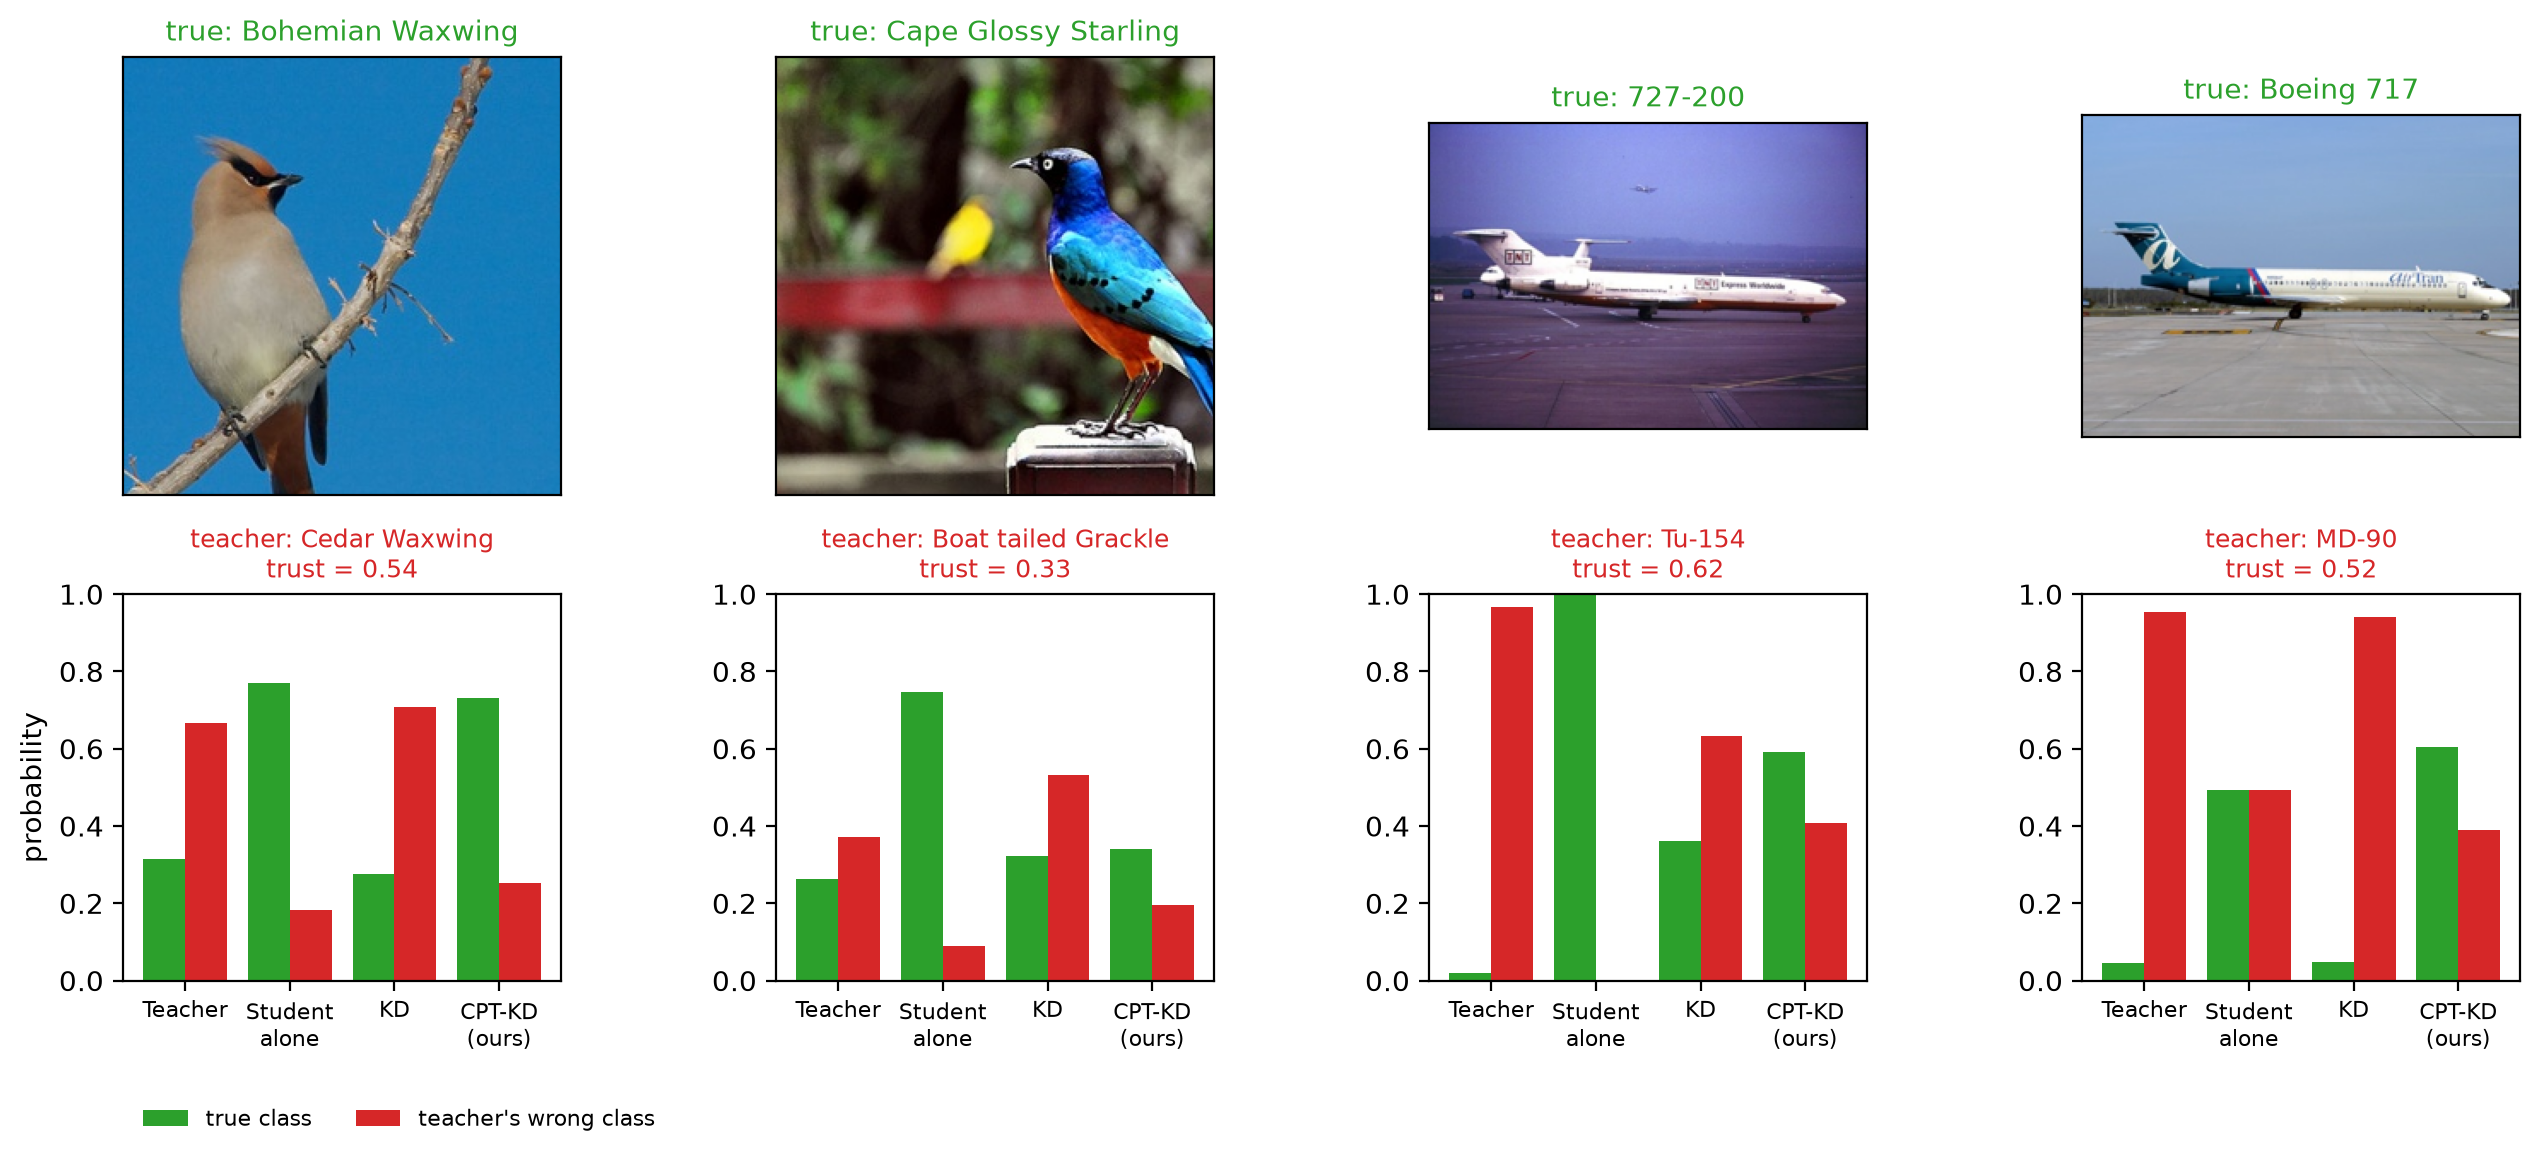
\includegraphics[width=0.86\textwidth]{figs/fig_problem.png}\\[-0.3em]
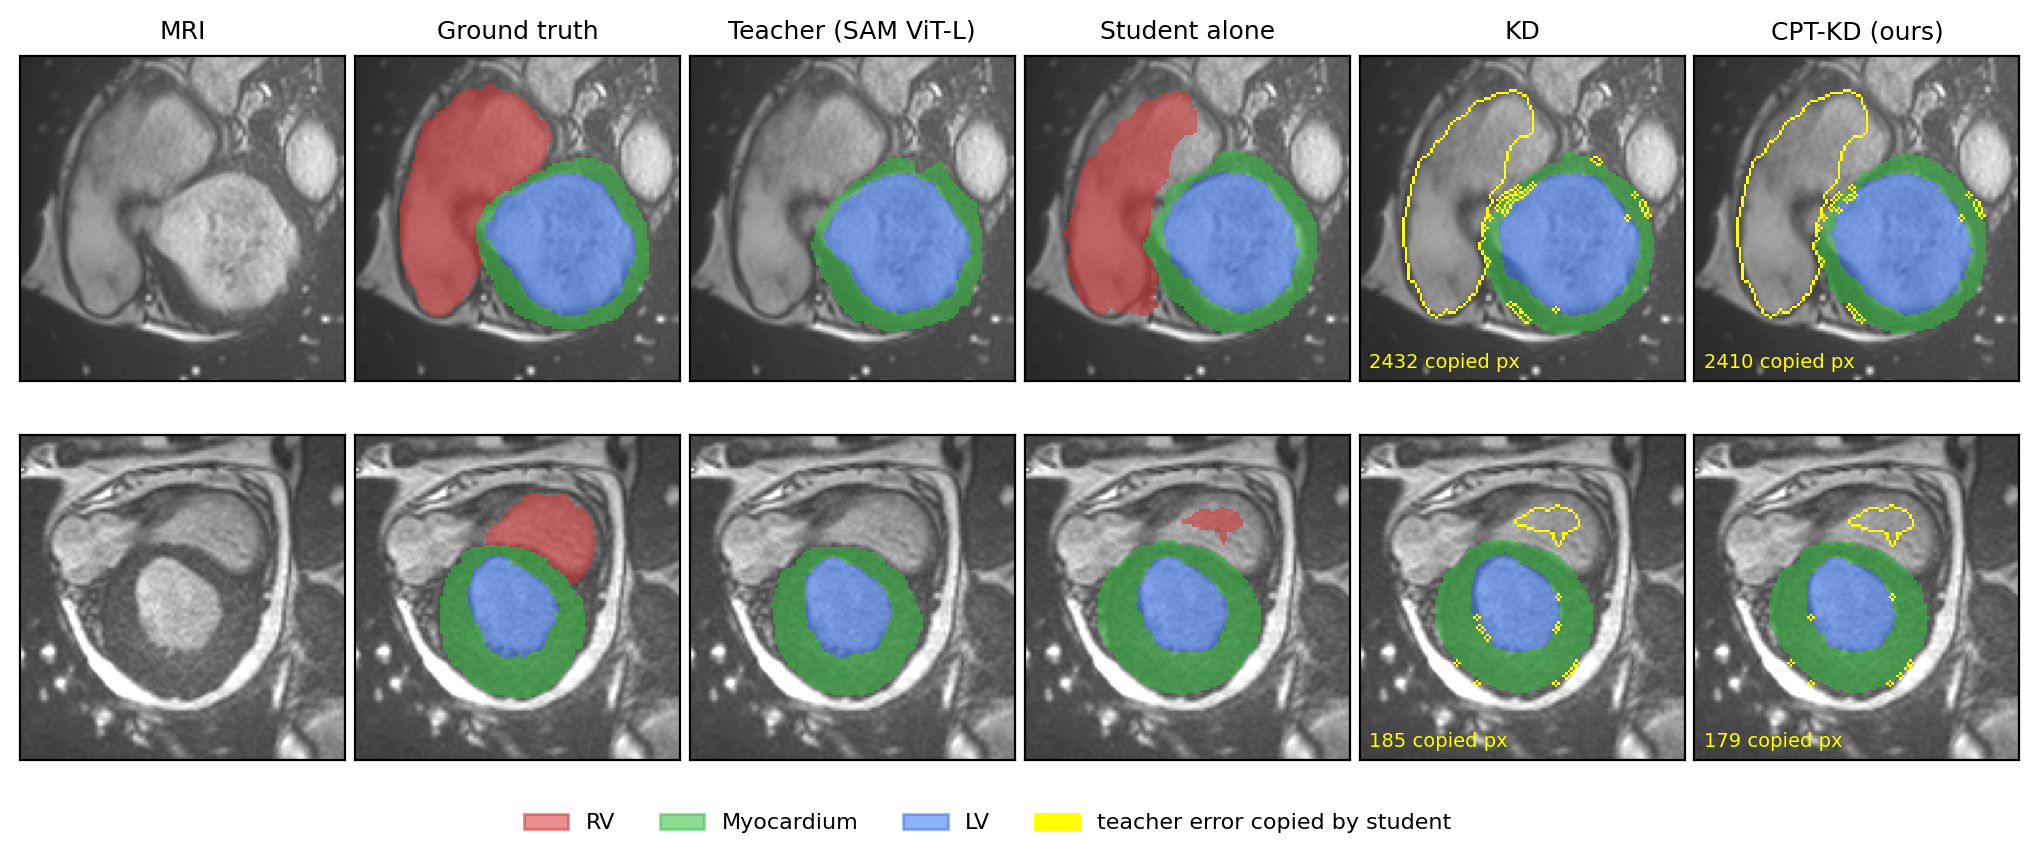
\includegraphics[width=0.70\textwidth]{figs/fig_problem_acdc.png}
\captionof{figure}{\textbf{The problem: a distilled student copies the teacher's look-alike confusions.}
\emph{Top:} real test images from CUB-200-2011 and FGVC-Aircraft. The ResNet-50 teacher confidently predicts a look-alike class (red), a ResNet-18 trained alone is right (green), and after vanilla KD the same student copies the teacher's mistake. CPT-KD, which turns down the teacher's soft label on low-trust class pairs, gives the right answer again.
\emph{Bottom:} the same effect in medical segmentation (ACDC cardiac MRI, SAM ViT-L teacher $\to$ EfficientNet-B1 student). Yellow outlines mark pixels where the teacher is wrong, the student alone is right, and the distilled student copies the teacher's error (\eg the missed right ventricle in row 1). This boundary-type error has trust 1, so CPT-KD copies it too (\cref{sec:seg}).}
\label{fig:teaser}
\end{center}
\vspace{0.6em}
}]

%%%%%%%%%%%%%%%%%%%%%%%%%%%%%%%%%%%%%%%%%%%%%%%%%%%%%%%%%%%%%%%%%%%%%%%%%%%%%%%%%%%%%%%%%%%%%
\begin{abstract}
Knowledge distillation (KD) trains a small student to match a large teacher's soft labels. Those soft labels also carry the teacher's \emph{confusions between look-alike classes}, and the student copies them even where it would have been right on its own. We measure this leak with \emph{teacher-error inheritance}: of the test images the teacher gets wrong, the share on which the student makes the same mistake. On CUB-200-2011 and FGVC-Aircraft, vanilla KD raises inheritance from 38.7\% to 47.4\% and from 31.5\% to 36.6\% (ResNet-50$\to$ResNet-18), even though the teacher makes no errors on its training images. We propose \textbf{Class-Pair Trust KD (CPT-KD)}. It estimates, from cross-fitted out-of-fold predictions, how much more the teacher confuses each class pair than a student trained alone, and scales down the teacher's soft label on exactly those pairs. CPT-KD needs about 20 lines of code and no new parameters. Over 2 datasets, 2 students and 3 seeds, it keeps KD's accuracy (within 0.5 points) and cuts inheritance on the flagged look-alike pairs by 4--10 points, below the level of a student trained alone. No baseline (DKD, weighted soft labels, Knowledge Adjustment, per-image gating, class-level trust) does this, and the reduction is significant by paired bootstrap in three of four setups. It closes only about a quarter of KD's \emph{overall} inheritance gap, where weighted soft labels do as well, and we explain why. CPT-KD does \emph{not} raise accuracy: the student falls back to its own errors rather than the right answer, and neither ensembles, combinations with WSL or a pair penalty, nor 20\% label noise change this. As a step beyond the proposal, we carry the analysis to medical image segmentation with a SAM foundation-model teacher. There the leak reappears and grows with the KD temperature, but CPT-KD has no measurable effect, because the errors lie on organ boundaries rather than between look-alike classes.
\end{abstract}

%%%%%%%%%%%%%%%%%%%%%%%%%%%%%%%%%%%%%%%%%%%%%%%%%%%%%%%%%%%%%%%%%%%%%%%%%%%%%%%%%%%%%%%%%%%%%
\section{Introduction}
\label{sec:intro}
Knowledge distillation~\cite{hinton2015distilling} is the standard way to obtain a compact model: the student minimises
\begin{equation}
\mathcal{L}_{\mathrm{KD}} = \mathrm{CE}(y, p_s) + \alpha\,\tau^2\,\mathrm{KL}\big(p_t^{\tau}\,\|\,p_s^{\tau}\big),
\label{eq:kd}
\end{equation}
where $p^{\tau}=\mathrm{softmax}(z/\tau)$. The \emph{dark knowledge} in $p_t^{\tau}$, the probability the teacher gives to wrong classes, is usually treated as uniformly useful. In fine-grained recognition this assumption is fragile. Bird species and aircraft variants differ in small details, so a teacher confuses particular look-alike pairs often and consistently, and Eq.~\eqref{eq:kd} passes these confusions on unchanged.

\cref{fig:teaser} shows the failure on real test images. A ResNet-50 teacher confuses a Bohemian Waxwing with a Cedar Waxwing and a Boeing~717 with an MD-90. A ResNet-18 trained alone gets these images right, but after KD the same ResNet-18 makes the teacher's mistake. Existing remedies act at the wrong level. Per-image methods~\cite{wen2021preparing,mishra2026correctness} only act when the teacher's top-1 prediction is wrong, which never happens on the teacher's own (memorised) training images. Weighted soft labels~\cite{zhou2021wsl} and class-level corrections~\cite{lukasik2022teacherspet} reweight whole images or classes, not individual class \emph{pairs}.

\paragraph{Research question.} Can the student keep the teacher's useful knowledge without inheriting its look-alike confusions?

\paragraph{Contributions.}
\begin{itemize}
\item[\textbf{C1}] \textbf{The hidden leak.} A teacher with zero training errors still raises teacher-error inheritance through its soft labels, on both fine-grained benchmarks and both students (\cref{sec:c1}).
\item[\textbf{C2}] \textbf{CPT-KD}, a drop-in change to the KD target: cross-fitted pair trust scores, followed by soft-label cleaning on low-trust pairs. It needs about 20 lines and no new parameters (\cref{sec:method}).
\item[\textbf{C3}] \textbf{How fine should trust be?} Per-image, per-class and per-pair trust compared under one recipe (\cref{sec:main}).
\item[\textbf{+}] \textbf{Beyond the proposal:} the analysis and CPT-KD carried over to medical image segmentation with a SAM foundation-model teacher~\cite{kirillov2023sam} on ACDC~\cite{bernard2018acdc} (\cref{sec:seg}), plus a released, reproducible code base.
\end{itemize}

%%%%%%%%%%%%%%%%%%%%%%%%%%%%%%%%%%%%%%%%%%%%%%%%%%%%%%%%%%%%%%%%%%%%%%%%%%%%%%%%%%%%%%%%%%%%%
\section{Related work}
\label{sec:related}
\paragraph{Soft-label distillation.} Vanilla KD~\cite{hinton2015distilling} matches temperature-softened outputs. DKD~\cite{zhao2022dkd} splits the KL term into a target part and a non-target part and up-weights the latter, so it trusts the wrong-class probabilities \emph{more}. Students do not simply become copies of teachers~\cite{stanton2021does}, and larger teachers do not always help~\cite{cho2019efficacy,mirzadeh2020takd}.

\paragraph{Correcting the teacher.} Knowledge Adjustment~\cite{wen2021preparing} swaps the top-1 and true-class probabilities when the teacher is wrong. Correctness-aware KD~\cite{mishra2026correctness} gates distillation per image by teacher correctness. Both act only on images where the teacher's top-1 prediction is wrong. Weighted soft labels (WSL)~\cite{zhou2021wsl} reweight each image by the student/teacher cross-entropy ratio. Lukasik \etal~\cite{lukasik2022teacherspet} show that distillation can hurt particular \emph{classes} and propose class-level corrections. Dao \etal~\cite{dao2021semiparametric} use cross-fitting to debias the teacher's predictions on its training data. We borrow cross-fitting to estimate \emph{pair-level} confusions. To our knowledge, CPT-KD is the first method to calibrate trust per (true class, wrong class) pair.

\paragraph{Distillation for segmentation.} Dense-prediction KD matches per-pixel distributions~\cite{shu2021cwd}. IAD~\cite{hong2026iad} distils a LoRA-adapted~\cite{hu2022lora} SAM~\cite{kirillov2023sam} into lightweight students for medical segmentation. We reuse its pipeline for our extension.

%%%%%%%%%%%%%%%%%%%%%%%%%%%%%%%%%%%%%%%%%%%%%%%%%%%%%%%%%%%%%%%%%%%%%%%%%%%%%%%%%%%%%%%%%%%%%
\section{Method: Class-Pair Trust KD}
\label{sec:method}
\paragraph{Idea.} Keep the teacher's soft label, but turn it down on the class pairs the teacher confuses \emph{more than a student trained alone}. A confusion the student would also make is not something KD adds, so we leave it alone. A confusion only the teacher makes is what the student would otherwise inherit.

\paragraph{Step 1: out-of-fold predictions.} The full teacher fits its training images perfectly (100\% training accuracy in our runs), so its training-set predictions reveal nothing about its confusions. Following cross-fitting~\cite{dao2021semiparametric}, we split the training pool into $K{=}5$ folds. For each fold $k$ we train a teacher and a student-alone on the other four folds and record their softmax outputs (temperature~1) on fold~$k$, which they never saw. The out-of-fold top-1 accuracy is 79.7\% (teacher) and 73.0\% (student) on CUB, and 78.0\% and 75.6\% on Aircraft.

\paragraph{Step 2: pair trust.} For true class $y$ and wrong class $c\neq y$, let $\bar p_t(c\,|\,y)$ and $\bar p_s(c\,|\,y)$ be the average out-of-fold probability that the teacher and the student-alone give to $c$ on training images of class~$y$. We define
\begin{equation}
\trust(y,c)=\min\!\Big(1,\;\frac{\bar p_s(c\,|\,y)+\epsilon}{\bar p_t(c\,|\,y)+\epsilon}\Big),\qquad \trust(y,y)=1,
\label{eq:trust}
\end{equation}
with $\epsilon=0.1/C$ for $C$ classes. A trust of 1 means the teacher is no more confused than the student on this pair. A trust near 0 means the confusion is the teacher's alone. We use averaged probabilities rather than error counts because there are only about 30 training images per class. \Cref{fig:trust} shows part of the CUB table. The lowest-trust pairs are genuine look-alikes (Fish Crow$\to$Common Raven, Forster's$\to$Common Tern, Sooty$\to$Laysan Albatross). Overall, 3.6\% of the CUB pairs and 7.2\% of the Aircraft pairs have trust $<0.5$.

\begin{figure}[t]
\centering
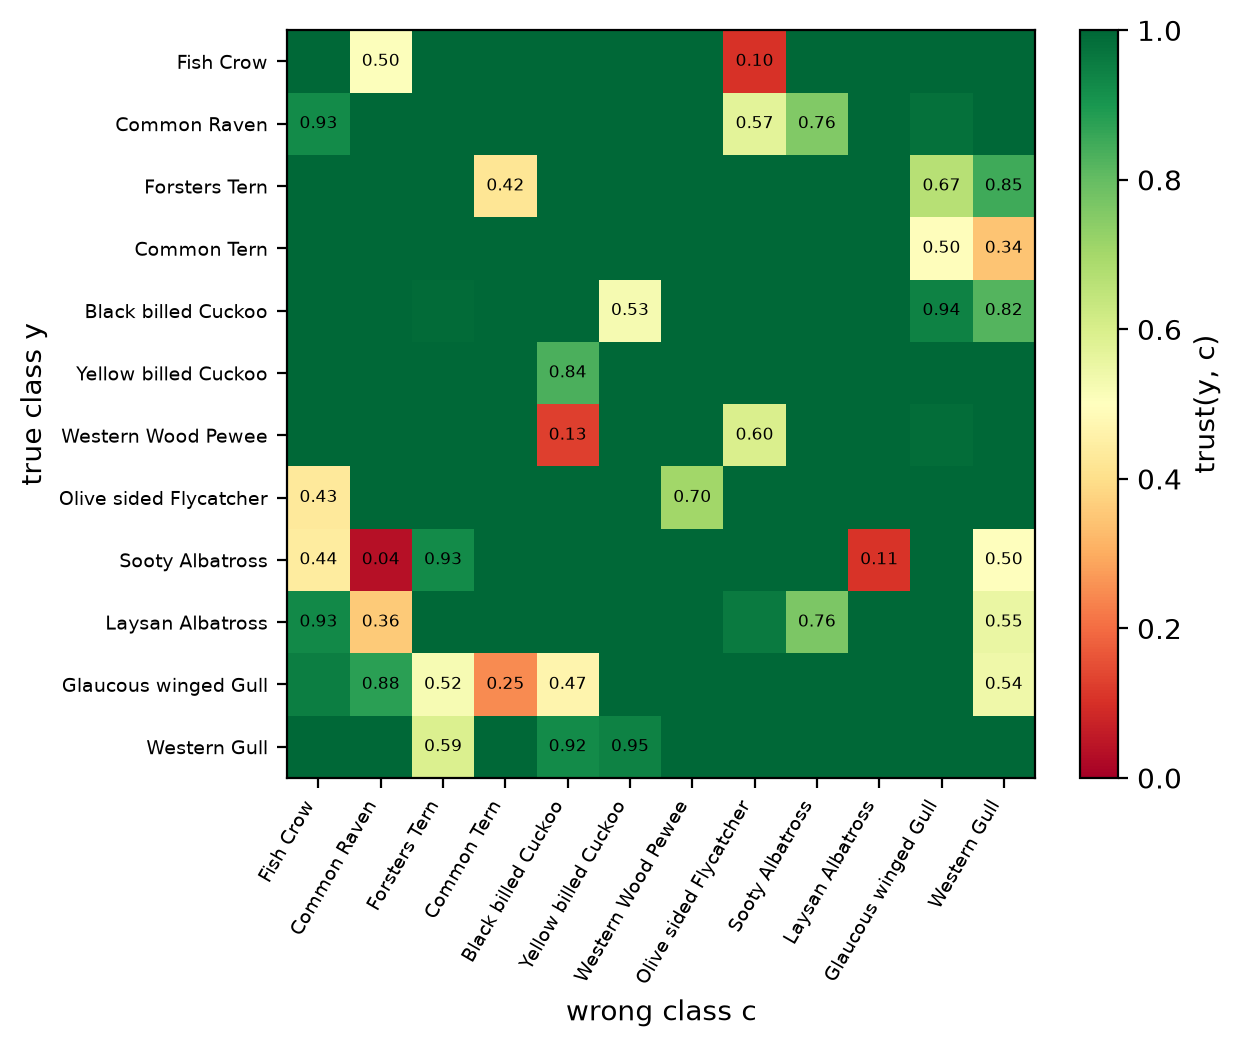
\includegraphics[width=0.72\linewidth]{figs/fig_trust_cub.png}
\caption{\textbf{Pair-trust table (CUB, Eq.~\ref{eq:trust})} over the classes in the lowest-trust pairs. Red cells are confusions made by the teacher only. They are look-alike species: crows and ravens, terns, albatrosses, gulls.}
\label{fig:trust}
\end{figure}

\paragraph{Step 3: clean the soft label.} For a training image with label $y$ and teacher soft label $q=p_t^{\tau}$ ($\tau{=}4$), we scale each wrong-class probability by its trust and rescale the wrong classes back to their original total, so the true-class probability is unchanged:
\begin{equation}
\tilde q_c = \frac{\trust(y,c)\,q_c}{\sum_{c'\neq y}\trust(y,c')\,q_{c'}}\,(1-q_y)\;\;(c\neq y),\qquad \tilde q_y=q_y .
\label{eq:clean}
\end{equation}
The student is then trained with Eq.~\eqref{eq:kd}, with $\tilde q$ in place of $p_t^{\tau}$. Mass removed from a teacher-only confusion moves to the wrong classes the teacher shares with the student, so the useful structure of the dark knowledge is kept. Keeping $q_y$ fixed avoids making the student over-confident. We ablate this choice in \cref{tab:ablation}. Unlike per-image methods, Eq.~\eqref{eq:clean} acts on \emph{every} training image, pair by pair. CPT-KD can also be combined with DKD by cleaning $q$ before the decoupling (``CPT-KD + DKD'').

%%%%%%%%%%%%%%%%%%%%%%%%%%%%%%%%%%%%%%%%%%%%%%%%%%%%%%%%%%%%%%%%%%%%%%%%%%%%%%%%%%%%%%%%%%%%%
\section{Experimental setup}
\label{sec:setup}
\paragraph{Datasets.} \textbf{CUB-200-2011}~\cite{wah2011cub}: 200 bird species, 5{,}994 training and 5{,}794 test images. \textbf{FGVC-Aircraft}~\cite{maji2013aircraft}: 100 variants (finest label level), 6{,}667 train+val and 3{,}333 test images, with the 20-pixel copyright banner removed. Images are resized to a shorter side of 256. Training uses a random 224 crop and horizontal flip; testing uses a center 224 crop. Settings were tuned on images held out from the training split (3 per class on CUB, the official val split on Aircraft). Final models are retrained on train+val and evaluated once on the official test split. No new data were collected. Both datasets are public research benchmarks without people as subjects. CUB contains a small share of mislabeled images~\cite{vanhorn2015building}, and some CUB images overlap ImageNet. This affects all methods equally.

\paragraph{Models and recipe.} The teacher is a ResNet-50~\cite{he2016resnet}. The students are ResNet-18 (same family) and MobileNetV2~\cite{sandler2018mobilenetv2} (cross-architecture). All networks start from torchvision ImageNet weights and use one recipe: SGD (Nesterov, momentum 0.9, lr 0.01, $10\times$ for the new head, weight decay $5\cdot10^{-4}$), batch 64, 40 epochs, linear warm-up then cosine decay, and bf16 mixed precision. KD uses $\tau{=}4$ and $\alpha{=}1$. DKD uses $\alpha{=}1$, $\beta{=}8$ and a 5-epoch warm-up. The teacher reaches 82.5\% (CUB) and 81.9\% (Aircraft) test accuracy. Each method is run with 3 seeds, and every method uses the \emph{same} seeds and the \emph{same} teacher. One student run takes 5--11 minutes on an RTX A5000/A6000.

\paragraph{Baselines.} (1) student alone (CE only); (2) vanilla KD~\cite{hinton2015distilling}; (3) DKD~\cite{zhao2022dkd}; (4) weighted soft labels~\cite{zhou2021wsl}; (5) Knowledge Adjustment~\cite{wen2021preparing}; (6) per-image correctness gate~\cite{mishra2026correctness}, which skips KD on images the teacher gets wrong; (7) class-level trust in the spirit of~\cite{lukasik2022teacherspet}, where one trust value per true class (the mean of its row of Eq.~\eqref{eq:trust}) scales all wrong-class probabilities. The full teacher is never wrong on its training images, so (6) would reduce to KD. We therefore give the gate the out-of-fold teacher predictions, which is the strongest fair version. Ours: (8) CPT-KD and (9) CPT-KD + DKD. Two further combinations were fixed in advance and run on ResNet-18 only: (10) CPT-KD + WSL (cleaned soft label, WSL per-image weight) and (11) CPT-KD + pair penalty, which adds $\lambda\sum_{c\neq y}(1-\trust(y,c))\,p_s(c)$ with $\lambda{=}1$ to push the student off teacher-only confusions.

\paragraph{Metrics.} Top-1 accuracy (CUB) and mean per-class accuracy (Aircraft, the official metric). \textbf{Teacher-error inheritance} ($\downarrow$): of the test images the teacher gets wrong, the percentage on which the student predicts the \emph{same} wrong class. \textbf{Flagged-pair inheritance} ($\downarrow$): the same, restricted to teacher errors $(y,\hat y_t)$ with $\trust(y,\hat y_t)<0.5$ (116 test images on CUB, 52 on Aircraft). Also reported: accuracy on teacher-correct images (a no-harm check), student--teacher agreement, expected calibration error (ECE, 15 bins)~\cite{guo2017calibration}, and worst-10-class accuracy.

%%%%%%%%%%%%%%%%%%%%%%%%%%%%%%%%%%%%%%%%%%%%%%%%%%%%%%%%%%%%%%%%%%%%%%%%%%%%%%%%%%%%%%%%%%%%%
\section{Results}
\label{sec:results}

\subsection{C1: the hidden leak}
\label{sec:c1}
\begin{figure*}[t]
\centering
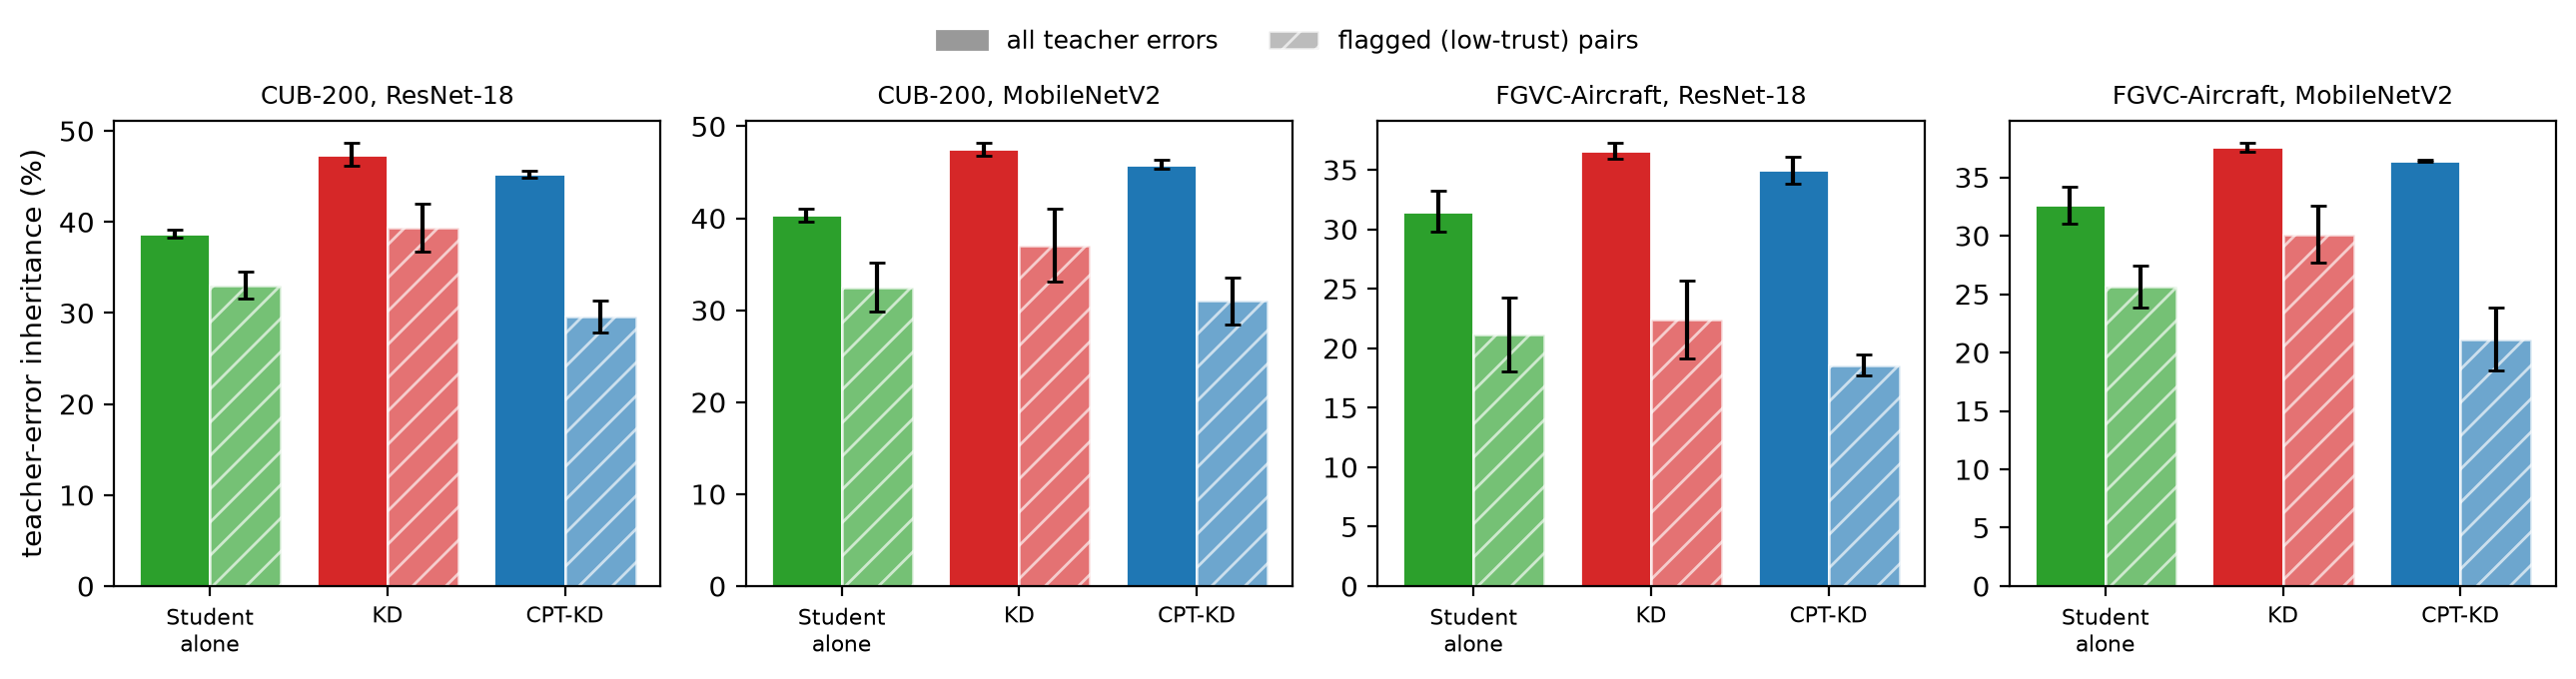
\includegraphics[width=0.92\textwidth]{figs/fig_c1_inheritance.png}
\caption{\textbf{Teacher-error inheritance} (\%, mean $\pm$ std over 3 seeds; lower is better). Solid bars: all teacher errors. Hatched bars: teacher errors on flagged (low-trust) pairs. KD (red) raises inheritance above a student trained alone (green) everywhere. CPT-KD (blue) brings flagged-pair inheritance below the student-alone level, but recovers only part of the overall increase.}
\label{fig:c1}
\end{figure*}
\Cref{fig:c1} (red vs.\ green bars) and the first two rows of \cref{tab:cub,tab:air} show that vanilla KD raises teacher-error inheritance in all four setups: 38.7$\to$47.4\% and 40.3$\to$47.5\% on CUB, 31.5$\to$36.6\% and 32.6$\to$37.6\% on Aircraft. Paired with the same seeds, the increase is $+8.7\pm1.8$ (CUB, ResNet-18) and $+5.1\pm2.7$ points (Aircraft, ResNet-18). This is far more than the variation between student-alone seeds. The teacher has 100\% training accuracy, so the leak cannot come from its top-1 mistakes on training images. It travels through the wrong-class probabilities of its soft labels. KD still helps overall (+3--4 points of accuracy), so the goal is to remove the leak, not KD.


\subsection{C2 and C3: main comparison}
\label{sec:main}
\Cref{tab:cub,tab:air} compare all nine methods.

\paragraph{Accuracy is kept.} CPT-KD is at most 0.5 points below vanilla KD in every setup. The gap is within one standard deviation for three of the four, while CUB/MobileNetV2 shows a small but consistent $-0.5$. All distillation methods beat the student alone by 3--4.5 points.

\paragraph{The targeted confusions are removed.} On flagged pairs, CPT-KD lowers inheritance compared with KD on the same seeds by $-9.8\pm1.3$ (CUB, R18), $-6.0\pm4.5$ (CUB, MNv2), $-3.9\pm3.3$ (Aircraft, R18) and $-9.0\pm2.2$ points (Aircraft, MNv2). In all four setups the result is \emph{below} the student-alone level (\eg 29.6\% vs.\ 33.0\% on CUB/R18). No baseline achieves this: none lowers flagged-pair inheritance by more than 3.5 points relative to KD, and some raise it. DKD, which up-weights the non-target distribution, \emph{increases} inheritance everywhere (\eg 49.9\% vs.\ 47.4\%), which is consistent with our diagnosis.

\paragraph{Overall inheritance falls only partly.} CPT-KD lowers overall inheritance by 1.2--2.1 points, about 25\% of the KD-induced increase. Most of KD's extra inheritance happens on pairs where the student-alone shows the same confusion ($\trust\approx1$), so these are \emph{shared} errors that CPT-KD leaves untouched by design. The rest reflects the general tendency of distilled students to agree with their teacher~\cite{stanton2021does}: agreement rises from 79.2\% (student alone) to 84.9\% (KD) and is 84.3\% for CPT-KD on CUB/R18. Weighted soft labels~\cite{zhou2021wsl} lower overall inheritance by about as much ($-1.3$ to $-2.6$ points), and significantly in all four setups (\cref{tab:boot}), so for the \emph{overall} leak WSL is at least as effective as CPT-KD. It does not, however, reduce inheritance on the flagged pairs in any setup.

\paragraph{C3: granularity of trust.} Per-image gating lowers overall inheritance (45.2\% on CUB/R18) but costs 1.6 points of accuracy (3.8 on Aircraft, ResNet-18), because it discards all KD signal on hard images, useful knowledge included. Class-level trust keeps accuracy but barely changes inheritance ($-0.6$ on CUB/R18, $-1.2$ flagged). Scaling a whole row cannot separate a teacher-only confusion from the useful dark knowledge in the same row. Pair-level trust is the only granularity that removes the targeted confusions without an accuracy cost.

\paragraph{Statistical significance.} Because the flagged sets are small, we test the differences to KD with a paired bootstrap over test images. Each of 1{,}000 resamples recomputes every metric for all three seeds and records the seed mean (\texttt{cls/bootstrap\_ci.py}, \cref{tab:boot}). CPT-KD's flagged-pair reduction is significant (95\% interval excludes 0) in three of four setups, but not on Aircraft/ResNet-18. Neither WSL nor class-level trust is significant on flagged pairs in any setup. CPT-KD's overall-inheritance reduction is significant on CUB but not on Aircraft. Its accuracy cost is significant only on CUB/MobileNetV2 ($-0.5$).

\begin{table}[t]
\centering\scriptsize
\setlength{\tabcolsep}{2pt}
\caption{\textbf{Paired bootstrap} (1{,}000 resamples of the test images, seed-averaged): difference to KD with 95\% interval. $^*$: interval excludes 0. Acc.\ is top-1 (CUB) or mean per-class (Aircraft).}
\label{tab:boot}
\resizebox{\linewidth}{!}{\begin{tabular}{ll ccc}
\toprule
Setup & Method $-$ KD & $\Delta$Acc. & $\Delta$Inh. & $\Delta$Flag. \\
\midrule
CUB, R18 & CPT-KD & -0.2 [-0.6, +0.1] & -2.1 [-3.6, -0.6]$^*$ & -9.8 [-14.8, -5.5]$^*$ \\
 & WSL & -0.0 [-0.4, +0.3] & -1.7 [-2.8, -0.5]$^*$ & -3.4 [-7.4, +0.4] \\
 & Class trust & +0.2 [-0.1, +0.5] & -0.6 [-1.9, +0.7] & -1.1 [-5.1, +3.0] \\
\midrule
CUB, MNv2 & CPT-KD & -0.5 [-0.9, -0.1]$^*$ & -1.6 [-3.2, -0.2]$^*$ & -6.0 [-10.3, -2.3]$^*$ \\
 & WSL & +0.1 [-0.2, +0.4] & -1.3 [-2.6, -0.2]$^*$ & +0.3 [-3.3, +3.7] \\
 & Class trust & -0.0 [-0.3, +0.3] & +0.1 [-1.0, +1.3] & -1.4 [-4.4, +1.5] \\
\midrule
Aircraft, R18 & CPT-KD & -0.2 [-0.7, +0.4] & -1.6 [-3.5, +0.2] & -3.8 [-8.9, +1.4] \\
 & WSL & -0.1 [-0.6, +0.4] & -2.0 [-3.9, -0.3]$^*$ & -0.0 [-5.0, +5.1] \\
 & Class trust & +0.1 [-0.4, +0.6] & -1.0 [-3.0, +0.7] & +2.6 [-3.8, +9.0] \\
\midrule
Aircraft, MNv2 & CPT-KD & -0.1 [-0.6, +0.4] & -1.2 [-3.0, +0.8] & -9.0 [-16.3, -1.7]$^*$ \\
 & WSL & +0.6 [+0.1, +1.1]$^*$ & -2.6 [-4.6, -0.5]$^*$ & -1.9 [-8.6, +4.3] \\
 & Class trust & -0.1 [-0.5, +0.4] & +0.6 [-1.3, +2.5] & -0.6 [-6.5, +5.3] \\
\bottomrule
\end{tabular}
}
\end{table}

\begin{table*}[t]
\centering\footnotesize\setlength{\tabcolsep}{4pt}
\caption{\textbf{CUB-200-2011} test results (mean $\pm$ std, 3 seeds). Inh.: teacher-error inheritance; Flag.: inheritance on flagged (low-trust) pairs; both in \%, lower is better. Teacher (ResNet-50): 82.5\% top-1.}
\label{tab:cub}
\begin{tabular}{l ccc ccc}
\toprule
 & \multicolumn{3}{c}{ResNet-50 $\to$ ResNet-18} & \multicolumn{3}{c}{ResNet-50 $\to$ MobileNetV2} \\
\cmidrule(lr){2-4}\cmidrule(lr){5-7}
Method & Top-1$\uparrow$ & Inh.$\downarrow$ & Flag.$\downarrow$ & Top-1$\uparrow$ & Inh.$\downarrow$ & Flag.$\downarrow$ \\
\midrule
Student alone & 76.6{\scriptsize$\pm$0.4} & 38.7{\scriptsize$\pm$0.5} & 33.0{\scriptsize$\pm$1.8} & 78.8{\scriptsize$\pm$0.1} & 40.3{\scriptsize$\pm$0.9} & 32.5{\scriptsize$\pm$3.3} \\
Vanilla KD~\cite{hinton2015distilling} & 80.7{\scriptsize$\pm$0.3} & 47.4{\scriptsize$\pm$1.6} & 39.4{\scriptsize$\pm$3.3} & 81.7{\scriptsize$\pm$0.0} & 47.5{\scriptsize$\pm$0.9} & 37.1{\scriptsize$\pm$4.8} \\
DKD~\cite{zhao2022dkd} & 80.5{\scriptsize$\pm$0.0} & 49.9{\scriptsize$\pm$0.4} & 42.8{\scriptsize$\pm$0.5} & 81.5{\scriptsize$\pm$0.1} & 49.6{\scriptsize$\pm$0.2} & 38.5{\scriptsize$\pm$3.9} \\
Weighted soft labels~\cite{zhou2021wsl} & 80.7{\scriptsize$\pm$0.3} & 45.7{\scriptsize$\pm$0.7} & 35.9{\scriptsize$\pm$1.0} & 81.8{\scriptsize$\pm$0.3} & 46.2{\scriptsize$\pm$0.5} & 37.4{\scriptsize$\pm$2.8} \\
Knowledge Adjustment~\cite{wen2021preparing} & 80.8{\scriptsize$\pm$0.2} & 46.9{\scriptsize$\pm$1.4} & 37.9{\scriptsize$\pm$2.3} & 81.7{\scriptsize$\pm$0.1} & 46.5{\scriptsize$\pm$0.2} & 35.9{\scriptsize$\pm$2.8} \\
Per-image gate~\cite{mishra2026correctness} & 79.1{\scriptsize$\pm$0.1} & 45.2{\scriptsize$\pm$0.9} & 37.6{\scriptsize$\pm$1.3} & 80.7{\scriptsize$\pm$0.4} & 45.5{\scriptsize$\pm$0.9} & 37.4{\scriptsize$\pm$2.2} \\
Class-level trust~\cite{lukasik2022teacherspet} & 80.9{\scriptsize$\pm$0.2} & 46.8{\scriptsize$\pm$0.8} & 38.2{\scriptsize$\pm$1.8} & 81.7{\scriptsize$\pm$0.1} & 47.6{\scriptsize$\pm$0.2} & 35.6{\scriptsize$\pm$3.3} \\
\midrule
\textbf{CPT-KD (ours)} & 80.4{\scriptsize$\pm$0.2} & 45.3{\scriptsize$\pm$0.5} & 29.6{\scriptsize$\pm$2.2} & 81.2{\scriptsize$\pm$0.0} & 45.9{\scriptsize$\pm$0.6} & 31.0{\scriptsize$\pm$3.1} \\
\textbf{CPT-KD + DKD (ours)} & 80.2{\scriptsize$\pm$0.2} & 46.2{\scriptsize$\pm$0.5} & 29.3{\scriptsize$\pm$0.9} & 81.1{\scriptsize$\pm$0.2} & 47.5{\scriptsize$\pm$1.0} & 33.3{\scriptsize$\pm$3.3} \\
\textbf{CPT-KD + WSL (ours)} & 80.3{\scriptsize$\pm$0.2} & 44.7{\scriptsize$\pm$0.5} & 30.7{\scriptsize$\pm$2.6} & -- & -- & -- \\
\textbf{CPT-KD + pair penalty (ours)} & 80.2{\scriptsize$\pm$0.2} & 46.3{\scriptsize$\pm$0.9} & 33.0{\scriptsize$\pm$0.5} & -- & -- & -- \\
\bottomrule
\end{tabular}

\end{table*}

\begin{table*}[t]
\centering\footnotesize\setlength{\tabcolsep}{4pt}
\caption{\textbf{FGVC-Aircraft} test results (mean $\pm$ std, 3 seeds); mAcc = mean per-class accuracy (official metric). Teacher (ResNet-50): 81.9\% top-1. DKD on ResNet-18 had one diverging seed (high std).}
\label{tab:air}
\begin{tabular}{l ccc ccc}
\toprule
 & \multicolumn{3}{c}{ResNet-50 $\to$ ResNet-18} & \multicolumn{3}{c}{ResNet-50 $\to$ MobileNetV2} \\
\cmidrule(lr){2-4}\cmidrule(lr){5-7}
Method & mAcc$\uparrow$ & Inh.$\downarrow$ & Flag.$\downarrow$ & mAcc$\uparrow$ & Inh.$\downarrow$ & Flag.$\downarrow$ \\
\midrule
Student alone & 79.0{\scriptsize$\pm$0.4} & 31.5{\scriptsize$\pm$2.1} & 21.2{\scriptsize$\pm$3.8} & 79.8{\scriptsize$\pm$0.6} & 32.6{\scriptsize$\pm$1.9} & 25.6{\scriptsize$\pm$2.2} \\
Vanilla KD~\cite{hinton2015distilling} & 82.8{\scriptsize$\pm$0.2} & 36.6{\scriptsize$\pm$0.8} & 22.4{\scriptsize$\pm$4.0} & 84.1{\scriptsize$\pm$0.2} & 37.6{\scriptsize$\pm$0.5} & 30.1{\scriptsize$\pm$2.9} \\
DKD~\cite{zhao2022dkd} & 78.9{\scriptsize$\pm$4.7} & 38.6{\scriptsize$\pm$3.7} & 23.7{\scriptsize$\pm$4.4} & 83.2{\scriptsize$\pm$0.5} & 41.9{\scriptsize$\pm$0.9} & 32.7{\scriptsize$\pm$0.0} \\
Weighted soft labels~\cite{zhou2021wsl} & 82.8{\scriptsize$\pm$0.4} & 34.6{\scriptsize$\pm$1.4} & 22.4{\scriptsize$\pm$7.8} & 84.7{\scriptsize$\pm$0.4} & 35.0{\scriptsize$\pm$0.7} & 28.2{\scriptsize$\pm$2.9} \\
Knowledge Adjustment~\cite{wen2021preparing} & 82.8{\scriptsize$\pm$0.3} & 36.6{\scriptsize$\pm$1.6} & 21.2{\scriptsize$\pm$5.8} & 84.4{\scriptsize$\pm$0.6} & 37.5{\scriptsize$\pm$1.9} & 28.8{\scriptsize$\pm$6.9} \\
Per-image gate~\cite{mishra2026correctness} & 79.1{\scriptsize$\pm$0.2} & 37.1{\scriptsize$\pm$1.8} & 28.8{\scriptsize$\pm$9.6} & 80.2{\scriptsize$\pm$0.3} & 38.9{\scriptsize$\pm$1.9} & 32.1{\scriptsize$\pm$2.9} \\
Class-level trust~\cite{lukasik2022teacherspet} & 83.0{\scriptsize$\pm$0.4} & 35.5{\scriptsize$\pm$1.4} & 25.0{\scriptsize$\pm$1.9} & 84.1{\scriptsize$\pm$0.3} & 38.1{\scriptsize$\pm$1.3} & 29.5{\scriptsize$\pm$4.0} \\
\midrule
\textbf{CPT-KD (ours)} & 82.7{\scriptsize$\pm$0.1} & 35.0{\scriptsize$\pm$1.4} & 18.6{\scriptsize$\pm$1.1} & 84.0{\scriptsize$\pm$0.2} & 36.4{\scriptsize$\pm$0.1} & 21.2{\scriptsize$\pm$3.3} \\
\textbf{CPT-KD + DKD (ours)} & 81.7{\scriptsize$\pm$0.3} & 38.7{\scriptsize$\pm$0.6} & 19.9{\scriptsize$\pm$4.8} & 83.7{\scriptsize$\pm$0.1} & 38.8{\scriptsize$\pm$1.0} & 17.9{\scriptsize$\pm$5.9} \\
\bottomrule
\end{tabular}

\end{table*}

\subsection{No-harm checks, calibration and fairness}
For ResNet-18 (all values in \texttt{tables/tab\_extra.tex}): on images the teacher gets right, CPT-KD keeps 92.5\% (CUB) and 93.8\% (Aircraft) accuracy, against 92.9\% and 93.9\% for KD, so the useful knowledge survives. ECE is slightly worse than KD on both datasets (3.9 vs.\ 3.6 on CUB, 7.3 vs.\ 6.9 on Aircraft). Redistributing wrong-class mass leaves the student a little over-confident; temperature scaling~\cite{guo2017calibration} would correct this. Worst-10-class accuracy is unchanged within noise (40.9 vs.\ 40.2 on CUB).


\subsection{Ablations}
\Cref{tab:ablation} varies the cleaning rule on CUB/ResNet-18 and reports differences to KD on the same seeds. Keeping the true-class probability (Eq.~\ref{eq:clean}) beats letting the true class absorb the removed mass: it has a smaller accuracy cost ($-0.24$ vs.\ $-0.45$) and a larger flagged-pair reduction. Squaring the trust (a stronger turn-down) lowers overall inheritance more ($-3.6$) but costs a full point of accuracy. Trust estimated at the KD temperature ($\tau{=}4$, 3 seeds; compare with the ``rescale all'' row) flattens the pair differences: the flagged-pair effect shrinks from $-8.9$ to $-2.6\pm4.0$, so temperature~1 is the right choice. Combining with DKD preserves the flagged-pair benefit ($-10.1$) but not DKD's other properties.

\begin{table}[t]
\centering\scriptsize
\setlength{\tabcolsep}{2.5pt}
\caption{\textbf{Ablation} on CUB, ResNet-18: difference to vanilla KD on the same seeds (mean $\pm$ std). Negative $\Delta$Inh./$\Delta$Flag. is better.}
\label{tab:ablation}
\resizebox{\linewidth}{!}{\begin{tabular}{l c ccc}
\toprule
Variant (CUB, ResNet-18) & Seeds & $\Delta$Top-1 & $\Delta$Inh. & $\Delta$Flag. \\
\midrule
Rescale all classes (true class absorbs mass) & 3 & -0.45{\scriptsize$\pm$0.42} & -1.65{\scriptsize$\pm$1.92} & -8.91{\scriptsize$\pm$2.49} \\
Keep true-class prob. (\textbf{default}) & 3 & -0.24{\scriptsize$\pm$0.32} & -2.14{\scriptsize$\pm$1.25} & -9.77{\scriptsize$\pm$1.32} \\
trust$^2$, rescale all & 3 & -1.01{\scriptsize$\pm$0.35} & -3.55{\scriptsize$\pm$1.94} & -9.77{\scriptsize$\pm$1.32} \\
trust$^2$, keep true class & 3 & -0.97{\scriptsize$\pm$0.20} & -2.63{\scriptsize$\pm$1.14} & -10.34{\scriptsize$\pm$5.24} \\
Trust estimated at $\tau{=}4$ (1 seed) & 1 & +0.36 & +0.20 & -6.03 \\
Per-class trust (keep true class) & 3 & +0.21{\scriptsize$\pm$0.18} & -0.63{\scriptsize$\pm$2.37} & -1.15{\scriptsize$\pm$2.17} \\
CPT-KD + DKD & 3 & -0.43{\scriptsize$\pm$0.33} & -1.22{\scriptsize$\pm$1.81} & -10.06{\scriptsize$\pm$4.07} \\
\bottomrule
\end{tabular}
}
\end{table}

\subsection{Can CPT-KD raise accuracy?}
\label{sec:acc}
CPT-KD lowers flagged-pair inheritance by up to 10 points, yet accuracy does not rise. \Cref{tab:errorflow} shows why. On the flagged images, the student rarely switches to the true class. Instead, the share of \emph{other} wrong answers rises by 3--7 points: the student falls back to its own mistakes. The correct share rises by up to 3 points in three of four setups, but these images are only 2\% of the test set (116/5{,}794 and 52/3{,}333). Inherited errors and accuracy are therefore separate problems: removing a copied error does not supply the missing correct knowledge.

We tested six further routes to an accuracy gain, all fixed before seeing test results. (i)~Letting the true class absorb the removed mass costs 0.45 points (\cref{tab:ablation}). (ii)~Squared trust costs 1.0 point. (iii)~Two-student ensembles: KD+CPT-KD is no better than KD+KD, and the share of images both students get wrong is unchanged (16.1 vs.\ 16.2\% on CUB/R18), so the changed errors are too few to diversify an ensemble (\cref{tab:errorflow}, right). (iv)~CPT-KD + WSL gives the lowest overall inheritance on CUB (44.7\%) but no accuracy gain ($-0.4$ on CUB, $-0.1$ on Aircraft). (v)~CPT-KD + pair penalty is inconsistent: $-0.5\pm0.4$ on CUB and $+0.4\pm0.5$ on Aircraft, and it weakens the flagged-pair effect. (vi)~With 20\% symmetric label noise (\cref{tab:noise}), where the teacher's errors are far more frequent, KD still gives $+7.5$/$+8.5$ points over the student alone, and CPT-KD stays $0.6$ below KD on both datasets. It still lowers flagged-pair inheritance (36.0$\to$31.6 and 24.9$\to$21.3), so the method is robust to noise in what it targets. The noisy trust table, however, flags 2.7$\times$ more pairs on CUB and so also removes some useful knowledge.

\begin{table*}[t]
\centering\footnotesize\setlength{\tabcolsep}{4pt}
\caption{\textbf{Where do the removed mistakes go?} Left/middle: on flagged test images (teacher wrong on a low-trust pair), the share the student gets right and the share it assigns to a third, wrong class (mean over 3 seeds; the rest copy the teacher). Right: accuracy of two-student ensembles (equal-weight average of two seeds).}
\label{tab:errorflow}
\begin{tabular}{l ccc ccc ccc}
\toprule
 & \multicolumn{3}{c}{Flagged: correct (\%)} & \multicolumn{3}{c}{Flagged: other wrong (\%)} & \multicolumn{3}{c}{2-student ensemble acc.} \\
\cmidrule(lr){2-4}\cmidrule(lr){5-7}\cmidrule(lr){8-10}
Setup & alone & KD & CPT & alone & KD & CPT & KD+KD & KD+CPT & CPT+CPT \\
\midrule
CUB, R18 & 25.6 & 29.3 & 32.2 & 41.4 & 31.3 & 38.2 & 81.35 & 81.16 & 80.97 \\
CUB, MNv2 & 25.3 & 31.9 & 30.7 & 42.2 & 31.0 & 38.2 & 82.46 & 82.14 & 81.56 \\
Aircraft, R18 & 21.2 & 25.0 & 25.6 & 57.7 & 52.6 & 55.8 & 83.35 & 83.60 & 83.29 \\
Aircraft, MNv2 & 23.1 & 27.6 & 30.8 & 51.3 & 42.3 & 48.1 & 85.04 & 84.90 & 85.12 \\
\bottomrule
\end{tabular}

\end{table*}

\begin{table}[t]
\centering\scriptsize
\setlength{\tabcolsep}{2.4pt}
\caption{\textbf{20\% symmetric label noise} on the training labels (test labels clean), ResNet-18, 3 seeds. Trust tables and teachers are rebuilt from the noisy labels.}
\label{tab:noise}
\resizebox{\linewidth}{!}{\begin{tabular}{l ccc ccc}
\toprule
 & \multicolumn{3}{c}{CUB, 20\% noise} & \multicolumn{3}{c}{Aircraft, 20\% noise} \\
\cmidrule(lr){2-4}\cmidrule(lr){5-7}
Method & Top-1$\uparrow$ & Inh.$\downarrow$ & Flag.$\downarrow$ & mAcc$\uparrow$ & Inh.$\downarrow$ & Flag.$\downarrow$ \\
\midrule
Student alone & 62.4{\scriptsize$\pm$0.3} & 24.1{\scriptsize$\pm$1.3} & 25.7{\scriptsize$\pm$1.4} & 61.6{\scriptsize$\pm$0.7} & 23.1{\scriptsize$\pm$0.6} & 14.6{\scriptsize$\pm$2.2} \\
Vanilla KD & 69.9{\scriptsize$\pm$0.2} & 34.3{\scriptsize$\pm$0.3} & 36.0{\scriptsize$\pm$0.6} & 70.1{\scriptsize$\pm$0.6} & 30.6{\scriptsize$\pm$0.4} & 24.9{\scriptsize$\pm$3.3} \\
\textbf{CPT-KD (ours)} & 69.2{\scriptsize$\pm$0.2} & 33.0{\scriptsize$\pm$0.6} & 31.6{\scriptsize$\pm$2.3} & 69.6{\scriptsize$\pm$0.6} & 30.0{\scriptsize$\pm$0.7} & 21.3{\scriptsize$\pm$4.4} \\
\bottomrule
\end{tabular}
}
\end{table}

\subsection{Error analysis}
The flagged pairs match expert intuition: Fish Crow/Common Raven, Forster's/Common Tern, Black-/Yellow-billed Cuckoo and Glaucous-winged/Western Gull on CUB; DC-10/MD-11, 737-500/737-300, A340-300/A340-200 and E-195/E-190 on Aircraft. A few implausible pairs (\eg 757-200$\to$A321) rest on only a few teacher mistakes, the expected noise from 30--67 training images per class.

%%%%%%%%%%%%%%%%%%%%%%%%%%%%%%%%%%%%%%%%%%%%%%%%%%%%%%%%%%%%%%%%%%%%%%%%%%%%%%%%%%%%%%%%%%%%%
\section{Beyond the proposal: medical segmentation}
\label{sec:seg}
Does the leak, and CPT-KD's remedy, carry over to dense prediction with a foundation-model teacher? We use the ACDC cardiac MRI benchmark~\cite{bernard2018acdc}: 4 classes (background, right ventricle RV, myocardium Myo, left ventricle LV), 1{,}304 training and 182 validation slices, and 40 test volumes (416 slices). We follow the IAD pipeline~\cite{hong2026iad}. The teacher is SAM ViT-L~\cite{kirillov2023sam} with rank-8 LoRA~\cite{hu2022lora} (91.2 test Dice). The student is an EfficientNet-B1~\cite{tan2019efficientnet} encoder with a SAM-style decoder. Training uses 200 epochs, AdamW (lr $10^{-4}$, weight decay 0.1), batch 6 and bf16. The loss is the segmentation loss ($0.1\,$CE$\,+\,0.9\,$Dice) plus $\alpha{=}1$ times [pixel-wise KL at temperature $\tau$ + IAD's class-prototype term]. CPT-KD applies Eq.~\eqref{eq:clean} \emph{to every pixel}, using that pixel's ground-truth class. To avoid training five extra SAM teachers, the trust table is estimated on the held-out validation slices, which neither the teacher nor the student-alone has seen. This is a cheaper stand-in for cross-fitting.

\paragraph{Findings.} Three pairs get low trust: RV$\to$LV (0.40), LV$\to$BG (0.49) and LV$\to$RV (0.10). These are confusions the SAM teacher makes but the small student does not. \Cref{tab:acdc} and \cref{fig:teaser} (bottom) show the results.
(i)~\textbf{C1 holds in segmentation.} On pixels where the teacher is wrong, inheritance rises from 56.5\% (student alone) to 58.4\% with KD at $\tau{=}1$ and to 60.1\% at $\tau{=}2$. It grows with temperature, \ie with how much wrong-class mass the soft label carries. KD copies 26\% of the pixels where the teacher is wrong but the student alone is right; row~1 of \cref{fig:teaser} shows a right ventricle missed entirely by the teacher and then by the distilled student.
(ii)~\textbf{CPT-KD has little room to act.} Most teacher errors on ACDC are boundary errors between an organ and the background, and the trust for those pairs is $\approx1$. The flagged pairs cover only 1.5\% of the teacher's wrong pixels. During training, CPT-KD changes less than $10^{-4}$ of the soft-label mass (total variation). Accordingly, CPT-KD at $\tau{=}1$ is indistinguishable from KD: Dice 89.9 vs.\ 89.8 (88.5 vs.\ 88.4 per volume) and inheritance 59.4 vs.\ 58.4\%, both within the spread of two student-alone seeds (0.2 Dice, 0.8 inheritance points). Flagged-pixel inheritance rests on only 1{,}963 pixels and varies from 15.9 to 24.4\% between two student-alone seeds, so it cannot separate the methods. \Cref{fig:teaser} (bottom) shows why: the missed right ventricle is an RV$\to$background confusion, which the student-alone also makes partly, so $\trust(\text{RV},\text{BG}){=}1$ and CPT-KD copies it just like KD (2{,}410 vs.\ 2{,}432 pixels).
In the binary polyp benchmark of IAD, Eq.~\eqref{eq:clean} is exactly the identity: with one wrong class, rescaling to its original total changes nothing. \emph{Pair-level trust therefore pays off when errors fall between look-alike classes, not when they fall on object boundaries.} This tells a practitioner when to use CPT-KD.

\begin{table}[t]
\centering\scriptsize
\setlength{\tabcolsep}{2.4pt}
\caption{\textbf{ACDC} (SAM ViT-L $\to$ EfficientNet-B1). Dice: mean over RV/Myo/LV on the 416 test slices at $256^2$; vol.\ Dice: official per-volume protocol; Inh.: teacher-error inheritance over pixels; T-ok: pixel accuracy where the teacher is right. Mean $\pm$ std over the seeds listed; one seed per KD/CPT-KD configuration.}
\label{tab:acdc}
\resizebox{\linewidth}{!}{\begin{tabular}{l c ccccc}
\toprule
Method & seeds & Dice$\uparrow$ & vol.\ Dice$\uparrow$ & Inh.$\downarrow$ & Flag.$\downarrow$ & T-ok$\uparrow$ \\
\midrule
Teacher (SAM ViT-L) & 1 & 92.3 & 91.2 & -- & -- & -- \\
Student alone & 2 & 89.7{\scriptsize$\pm$0.2} & 88.2{\scriptsize$\pm$0.1} & 56.9{\scriptsize$\pm$0.6} & 20.2{\scriptsize$\pm$6.0} & 99.67{\scriptsize$\pm$0.00} \\
KD ($\tau{=}1$) & 1 & 89.8 & 88.4 & 58.4 & 2.9 & 99.67 \\
CPT-KD ($\tau{=}1$) & 1 & 89.9 & 88.5 & 59.4 & 32.9 & 99.69 \\
KD ($\tau{=}2$) & 1 & 89.6 & 88.0 & 60.1 & 14.9 & 99.68 \\
\bottomrule
\end{tabular}
}
\end{table}

%%%%%%%%%%%%%%%%%%%%%%%%%%%%%%%%%%%%%%%%%%%%%%%%%%%%%%%%%%%%%%%%%%%%%%%%%%%%%%%%%%%%%%%%%%%%%
\section{Limitations and honest assessment}
\label{sec:limits}
\begin{itemize}
\item \textbf{Partial, narrow fix.} CPT-KD removes teacher-only confusions but closes only about 25\% of KD's overall inheritance gap, where weighted soft labels do as well. Its effect is confined to the 1.6--2\% of test images with teacher-only confusions, so it does not raise accuracy (\cref{sec:acc}).
\item \textbf{Small flagged sets} (116 and 52 test images): the Aircraft/ResNet-18 reduction ($-3.8$, 95\% CI $[-8.9,+1.4]$) is not significant; the other three are. Accuracy cost is significant only on CUB/MobileNetV2 ($-0.5$); ECE is slightly higher.
\item \textbf{Not run} (time budget): the ResNet-101 teacher, 10\% label noise and 2- vs.\ 5-fold trust. On ACDC, trust is estimated on validation slices rather than cross-fitted, and each configuration has a single seed.
\end{itemize}

\section{Reproducibility statement}
\label{sec:repro}
Code, configurations, logs, per-run results, test logits and trust tables are at \repourl, with step-by-step commands in \texttt{README.md} and our declaration in \texttt{REPRODUCIBILITY.md}; the conda environments are in \texttt{environment/}. Every table is regenerated from the released files by \texttt{cls/make\_tables.py}, \texttt{cls/bootstrap\_ci.py}, \texttt{cls/error\_flow.py} and \texttt{seg/make\_acdc\_table.py}, and every figure by \texttt{cls/make\_figures.py} and \texttt{seg/make\_seg\_figure.py}. Seeds are fixed and all methods share the same teachers. Weights are too large for the repository; \texttt{checkpoints/README.md} lists their SHA-256 hashes and how to regenerate them.

\section{Conclusion}
Distilled students copy their teacher's look-alike confusions, even from a teacher that makes no training errors. We showed this on two fine-grained benchmarks and on medical segmentation with a SAM teacher. CPT-KD estimates which class pairs the teacher confuses more than a student would, and turns down only those pairs in the soft label. It removes the targeted confusions, bringing flagged-pair inheritance below the level of an independently trained student, while keeping KD's accuracy, in about 20 lines and with no new parameters. Its limits are equally clear: it cannot fix shared confusions or the student's general imitation of the teacher, and it needs errors between classes rather than on object boundaries.


{\small
\bibliographystyle{ieeenat_fullname}
\bibliography{main}
}
\end{document}
